%Introduction
\chapter{Introduction}
According to the U.S. Department of Energy \cite{DOE2010}, energy for heating and cooling accounts for approximately 35 - 45\% of the total expenditure within a building.  With such a large investment of energy being used to regulate the temperature of a building, possible areas of improvement are heavily sought after.  Fully automated buildings with control systems to automatically heat and cool individual rooms or spaces have been designed \cite{Controls2013, Controls2013a} to reduce building energy usage while maintaining proper temperatures throughout the building.  These systems are complex and require knowledge of room usage, and in more complex systems room occupancy, as inputs into system control models.
	
While many factors such as ambient temperature, ventilation air flow, room volume, \textit{etc.} affect the time it takes to heat or air condition a room, it still takes on the order of many minutes to bring a room to a stable desired temperature \cite{yang2004}.  Due to this lag in changing the temperature of a room, it is not sufficient for control systems to begin air conditioning a room upon initial occupancy.   Thus, to ensure that room temperatures are appropriate, smart building control systems typically rely on set schedules of occupancy.  These systems may use scheduled occupancy up to 24 hours into the future to determine current heating and air conditioning control \cite{Ma2010}.  

However, what happens to the system when building traffic deviates from its schedule?  Let us consider a university classroom building.  While not often, professors will occasionally cancel class.  What should a smart control system do during this time?  It does not make sense for the system to heat or cool the room as though it was occupied.  The system should adapt to the changing environment.  Similarly, what happens if snow has caused many of the students and faculty to stay at home?  In this case, a cancelled class in the morning is likely correlated to class cancellations later in the day.  Ideally the building control system should identify situations where there is a significant deviation in the number of occupants within any part of the building and modify its heating or cooling schedule to account for such situations.  In both of these scenarios, a set schedule is insufficient to produce an optimal heating or cooling schedule for the building.

As another example of the usage of complex control systems, consider the roadways of the United States.  Optimal timing of traffic lights on major roadways across the United States could result in approximately a 22\% reduction in emissions along with a 10\% reduction in fuel consumption \cite{DOT2007}.  As of 2005 the total estimated fuel savings would amount to approximately 17 billions gallons of motor fuels annually.  This traffic light timing does not only consider city lights, but also takes into account freeway onramp volume lights.

In the United States, traffic light timings are often determined by an individual from the local department of transportation standing near the light and manually determining a timing schedule, or in some cases multiple schedules to account for peak traffic times and non-peak times \cite{Koonce2008}.  These schedules are then fixed and are changed either when roadways change to make new timings necessary or if petitioned by local citizens.  These timings are then either set in local control box for that traffic light or by a central control system for the city.  

As with the building scenario, what happens when the traffic deviates from normal?  Fixed timings will not be able to account for changes in traffic.  Inclement weather scenarios should likely require different timings then sunny days.  Lights near large sporting events likely require different timings during those events than typical evenings.  Even if schedules were made for such scenarios, there certainly exist scenarios for which schedules can not be made manually such as lane blockages due to accidents. 

In both of the above environments, the control systems have to account for future occupancy of the environment.  It is inadequate for these systems to use only current data to control the system.  Accurate forecasts of the systems usage are necessary to produce optimal control systems.  

%Problem Statement
\subsection{Problem and Objective}
As alluded to with the above examples, our focus is on improving forecasting accuracy on human controlled traffic systems.  By “traffic”, we mean the movement of vehicles along a road network, the movement of people in a building, or similar data derived from the actions of a group of people.  Overall, our method is more general than just traffic systems and we believe it will work with any dataset which has rare repeated events that lead to similar effects in the system.  For the rest of this paper, we define a time series dataset as $\{x_{t}^{(m)}\}$.  Each $x_{t}^{m}$ is an aggregate of the readings from sensor $m$ reading at time block $t$.  Our objective in this work is then:

\begin{enumerate}
	\item Produce an accurate forecast for $x_{t}^{(m)}$ $\delta$ time steps into the future.
	\item Reduce worst case forecasts.
	\item Keep approach unsupervised.
\end{enumerate}

Because the literature on forecasting is so vast, we specifically focus only on human traffic systems.  As we will demonstrate shortly, our approach will make some assumptions based on the type of data produced by these traffic systems which will   As a result, we will demonstrate considerably better results that would likely be possible with data from other sources.  Also, we will demonstrate our results empirically.  Due our lack of theoretical constraints, our improved results may simply be a by product of our datasets and and not something that may be applicable to other human traffic systems.  Of course, we do not believe this to be the case due to the improvement in vastly different datasets which we will demonstrate later.


%Give a sample example of the broncos game here and then discuss the need for worst case forecasts.
\subsubsection{A motivating example}

To illustrate an example of the need to minimize worst case forecasts, we present the following example.  The Denver Broncos, as with most American Football teams are a significant local attraction.  In 2010 the team had an average attendance of 74,908 \cite{ESPN2013}.  This attendance, combined with additional fans flooding downtown to patronize bars and restaurants creates an interesting effect on freeway traffic patterns.  Unsurprisingly, prior to the game there is an increase in total traffic volume along a freeway which is near the Broncos' Stadium.  Also, there exists a nearly 20\% drop in total traffic volume along the same stretch of freeway during the game.  ~\ref{fig:broncos} shows the total counts of Denver traffic by a single loop detector on a stretch of highway near the station for each hour of the day averaged for the first four Sunday Broncos home games and for the first four Sunday away games in 2010.  Comparing ~\ref{fig:broncos_off} with figure~\ref{fig:broncos_on} it is evident that a noticeable change in traffic patterns occur from approximately noon until approximately 6:00 pm.  This traffic change corresponds with a 2:05pm kickoff time for the game.

\begin{figure}[!ht]
	\begin{center}
		\subfigure[] {
			\includegraphics[width=0.49\textwidth]{broncos_off4.png}
			\label{fig:broncos_off}
		}
		\subfigure[] {
			\includegraphics[width=0.49\textwidth]{broncos4.png}
			\label{fig:broncos_on}
		}
	\end{center}
	\caption{Total number of cars passing major highway sensors in Denver on Sundays in September and October 2010}
	\label{fig:broncos}
\end{figure}

Such a significant difference in traffic patterns should lead to a change in traffic light control.  We have all likely encountered the frustrating scenario of attempting to leave one of these sporting events.  Traffic lights are often still on predefined timings and the situation arises where a large number of vehicles attempt to get through a traffic light controlled intersection in one direction with almost no vehicles attempting to get through the intersection in the perpendicular direction.  Ideally the light timings should be changed to fix this scenario and increase the green light time in the direction with multiple cars.  Of course, optimally other light timings will also need to be changed to account for the increase volume of traffic along certain paths within the city.

Traditional parametric forecasting models have difficulty accounting for these different traffic patterns and the problem becomes more difficult when when it is considered that the Broncos may play a Sunday night game or a Monday night game.  Thus our another goal of our approach is to handle these significant deviations from normal traffic patterns which are typically the causes of worse case forecasting scenarios.


\subsection{Approach}
To satisfy our first objective of producing an accurate forecast for dataset $x_{t}^{(m)}$ $\delta$ time steps into the future, we have created an ensemble forecasting model based on the Bayesian combined forecaster (BCF) created by Petridis \cite{Petridis2001}.  Chapter \ref{ch:BCF} discusses modifications we have made to BCF which improve its performance on human controlled traffic systems.  

To satisfy our second objective of reducing worst case forecasts, i.e. the sporting event scenario, we introduce a novel forecasting technique based on anomaly detection and modeling.  Empirically we have found that for human controlled traffic systems large deviations in forecasting accuracy often coincided with human controlled activities.  For the purposes of this paper, we frequently interchange the terms activities and anomalies.  The reason for this is as a matter of perspective.  To a forecasting model, an infrequently occurring human activity will likely produce anomalous results.  We describe any event which causes large prediction errors for our forecasting system as either an anomaly or an activity.  For vehicle traffic systems these activities might be sporting events, road closures, or accidents.  In the case of building models, such activities might be large infrequent meetings, cancelled classes, or early closure due to holidays.

Because such activities can overlap or occur at different times with varying amount of background noise present, it is a difficult task for one parametric model to accurately encapsulate all of the activities which occur within the system.  Our approach is to split the problem of forecasting into two parts: development of a background model and the development of a set of activity models.  Our background model is represented by any forecasting model.  In practice we have computed our results using traditional forecasting models such as Time Delayed Neural Networks, Auto Regressive Models or Support Vector Machines.   

To model activities, we propose comparing different models from the activity recognition literature along with a new model which we propose here.  Forecasting is then performed using an ensemble predictor defined in Chapter 5, taking outputs from all trained activity models and the background model.  ~\ref{fig:alg_overview} shows the general structure of our approach.  We combine classic forecasting models with activity models in a novel ensemble model to improve overall forecasting accuracy.

\begin{figure}
	\centering
	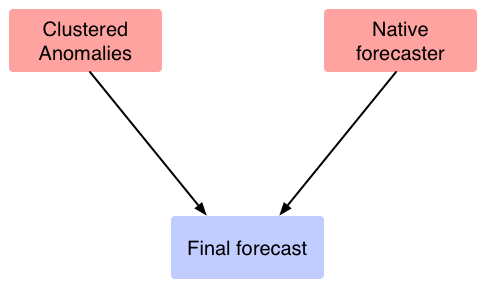
\includegraphics[width=0.5\textwidth]{simple_approach_overview.png}
	\caption{High level overview of our approach}
	\label{fig:alg_overview}
\end{figure}

Finally, in satisfying our third objective, we keep everything unsupervised.  Nothing in our approach prevents the use of supervised modeling of activities and incorporating a trained activity model into our final forecast, but such supervised information is not necessary to achieve improved forecasting results.


\subsection{Contributions}  
The contributions to the field of unsupervised traffic forecasting from this work are:
\begin{itemize}
\item{Extraction and modeling of forecasting activity models using residual errors from another forecasting model.}
\item{An improvement to a combined Bayesian prediction model to improve forecasting accuracy}
\item{A combined prediction model using an ensemble forecaster and activity models to improve short term forecasts during the presence of anomalous activities}
\end{itemize}

\subsection{Structure of the Thesis}
The remainder of this thesis is outlined as follows: Chapter 2 defines typical forecasting models which are to be used for comparison and as base native forecasters for our final ensemble forecaster.  This chapter also introduces some notation used through this document.  Chapter 3 discusses the datasets used therein along with specifics details on any necessary changes to make the datasets compatible with our forecasters.  Chapter 4 discusses a classic ensemble forecaster which we apply to our datasets along with introducing some improvements on this forecaster which greatly improve its long term forecasting performance.  Finally Chapter 5 discusses our novel approach using activity modeling to improve the short term accuracy of any of our base forecaster for our datasets.  This section also includes a brief discussion of previous work in the realm of anomaly detection.